\setcounter{subsection}{2}
\subsection{記憶域の割当とガベージコレクション}
5.4では, レジスターマシンを使ってSchemeの評価機を%
作成する. そのために, メモリーを抽象化した方が良いので,
リスト構造として表現したメモリーとそのメモリを操作するための%
抽象化を作る.

リストで表現したメモリを作るために, 主に2つの問題点がある.
\begin{enumerate}
\item コンピュータのメモリで表現できるものだけでどのように%
  リスト構造を表現することができるか.
\item メモリがなるべくいっぱいにならなようにどうすれば良いのか.
\end{enumerate}
%
まず1について説明し, そのあとガーベージコレクションの説明で%
2について説明する.
%
\subsubsection{ベクタとしてのメモリ}
コンピュータのメモリはユーニックなアドレスを持つブロックで分かれている.
基本的にブロックに値を入れるための操作とブロックからその値を取り出す%
ための操作が準備されていることが多い. また, メモリのアドレスも
データとして扱われていて, そのアドレスで演算などを行うことができる.

メモリを表現するために, ベクターというデータ構造を用いる.
ベクターはコンパウンドデータで, 添字を用いて定数時間で要素を%
取り出せるようになっている. メモリの操作を表すために,
次の2つのプロシジャを用いる.

\begin{lstlisting}[basicstyle=\footnotesize]
(vector-ref <vector> <n>)
(vector-set! <vector> <n> <value)
\end{lstlisting}
\paragraph{Lispのデータ構造の表現}
ベクターを用いてリスト構造に使うペアを表すことができる.
メモリが\lstinline{the-cars}と\lstinline{the-cdrs}という2つの%
ベクターで分かれているとする. ペアはその2つのベクターの添字として%
表すことができる. また, 数字や記号を表す方法も必要となる. そのために,
型のついたポインターを用いることができる. 例えば, \lstinline{n4}は
4という整数を表し, \lstinline{p5}はインデックス5のペアを表す. また,
\lstinline{e0}は空のリストを表す.
%
\begin{figure}[h]
  \centering
  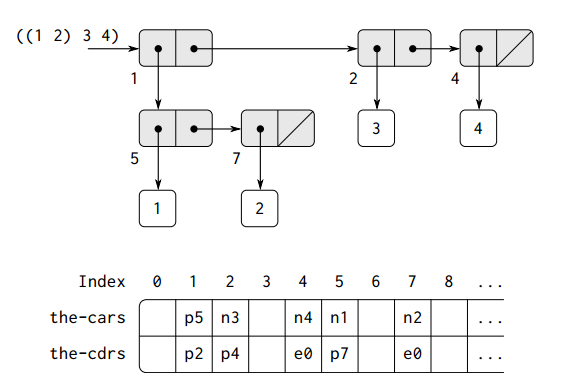
\includegraphics[height=6cm,width=12cm]{imgs/box-and-pointer.png}
\end{figure}
%
\paragraph{リストの基本操作}
操作を実装するために, \lstinline{the-cars}と\lstinline{the-cdrs}レジスターを用いる.
また, \lstinline{vector-ref}と\lstinline{vector-set!}という操作が使えることを%
前提とする. それを用いて,
%
\begin{lstlisting}[basicstyle=\footnotesize]
(assign <reg 1 > (op car) (reg <reg 2 >))
(assign <reg 1 > (op cdr) (reg <reg 2 >))
\end{lstlisting}
%
を次のように実装できる.
%
\begin{lstlisting}[basicstyle=\footnotesize]
(assign <reg 1 > (op vector-ref) (reg the-cars) (reg <reg 2 >))
(assign <reg 1 > (op vector-ref) (reg the-cdrs) (reg <reg 2 >))
\end{lstlisting}

\lstinline{set-car!}と\lstinline{set-cdr!}についても同じく実装できる.

また, 次に使える添字を常に指している\lstinline{free}というレジスターが%
存在するとする. それらを用いて,

\begin{lstlisting}[basicstyle=\footnotesize]
(assign <reg 1 > (op cons) (reg <reg 2 >) (reg <reg 3 >))
\end{lstlisting}
を次のように実装できる.
\begin{lstlisting}[basicstyle=\footnotesize]
(perform
  (op vector-set!) (reg the-cars) (reg free) (reg <reg 2 >))
(perform
  (op vector-set!) (reg the-cdrs) (reg free) (reg <reg 3 >))
(assign <reg 1 > (reg free))
(assign free (op +) (reg free) (const 1))
\end{lstlisting}

また, \lstinline{eq?}を次のように

\begin{lstlisting}[basicstyle=\footnotesize]
(op eq?) (reg <reg 1 >) (reg <reg 2 >)
\end{lstlisting}

で実装できる.
%
\subsubsection{無限のメモリの幻想を維持する}
以上紹介した構造では, リスト構造を表現することができるが,
メモリーが無限にあるという前提になってしまう. 実際の%
コンピュータでは, メモリが有限なので, メモリを使い切らない方法%
を考える必要がある. そのために, 使わなくなった結果などを消して%
そのメモリの部分を再利用できるようにする. その方法は
ガーベージコレクションという.

\paragraph{stop-and-copyガーベージコレクター}
ここで, \lstinline{root}というレジスターが%
現在アクセスできるすべてのデータの情報を持つ%
データ構造を指しているとする.

メモリで2つで分ける. 現在使っているデータは%
\lstinline{the-cars}と\lstinline{the-cdrs}とし,
使われていないメモリは\lstinline{new-cars}と\lstinline{new-cdrs}とする.

現在使っているメモリがいっぱいになると, 使っているデータのみ
使われていないメモリにコピーし, 現在のメモリをすべて空にする.

\begin{figure}[h]
  \centering
  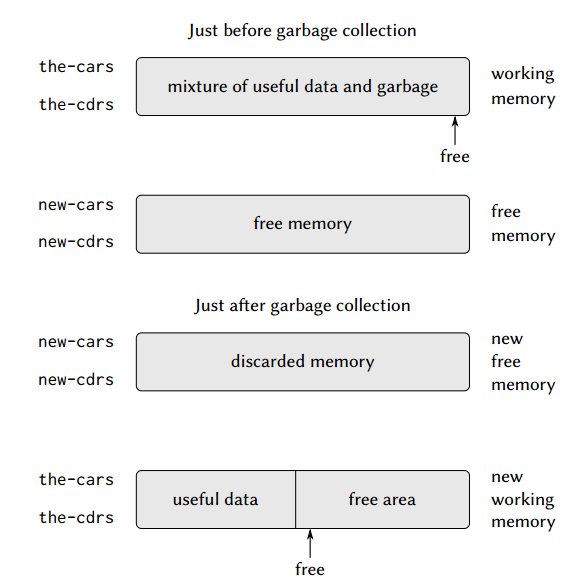
\includegraphics[height=6cm,width=8cm]{imgs/stop-and-copy.png}
\end{figure}

